\documentclass[11pt]{book}
\usepackage[slovene]{babel}
\usepackage[utf8]{inputenc}
\usepackage{amsmath}
\usepackage[dvipsnames]{xcolor}
\usepackage{titlesec}
% \usepackage{amssymb}
\usepackage{pstricks,pst-plot,pst-math}
\usepackage{pstricks-add}
\usepackage{graphicx}
\usepackage{enumerate}
\usepackage{color}
\usepackage{fouriernc}
\usepackage{microtype}
\usepackage{MnSymbol}
\usepackage{tikz-cd}
\usetikzlibrary{backgrounds}
\usepackage{wrapfig}
\usepackage{geometry}
\geometry{
    a4paper,
    left=45mm,
    right=45mm,
    top=20mm,
    bottom=20mm
    }
    \usepackage{comment}
    

\usepackage{amsthm}

\usepackage{changepage}   % for the adjustwidth environment
\usepackage{hyperref}
\hypersetup{
    colorlinks=true,
    linkcolor=cyan,
    filecolor=magenta,      
    urlcolor=cyan
    }

\usepackage[backgroundcolor=svetlosiva,linecolor=siva,textsize=footnotesize]{todonotes}

\pagestyle{plain}

\usepackage{enumitem}
\setlist[description]{leftmargin=\parindent,labelindent=\parindent, font=\normalfont\itshape\textbullet\space}


\def\NN{\mathbf{N}}
\def\ZZ{\mathbf{Z}}
\def\QQ{\mathbf{Q}}
\def\RR{\mathbf{R}}
\def\CC{\mathbf{C}}
\def\conclass{\mathcal{C}}
\def\11{\mathbf{1}}
\def\FF{\mathbf{F}}
\def\Fcal{\mathcal{F}}
\def\EE{\mathbf{E}}
\def\PP{\mathbf{P}}
\def\HH{\mathbf{H}}
\def\youngsym{\sigma_{\lambda}}

\DeclareMathOperator\image{im}
\DeclareMathOperator\sgn{sgn}
\DeclareMathOperator\Res{Res}
\DeclareMathOperator\Ind{Ind}
\DeclareMathOperator\Rep{Rep}
\DeclareMathOperator\mult{mult}
\DeclareMathOperator\Izotip{Izotip}
\DeclareMathOperator\MK{MK}
\DeclareMathOperator\tr{tr}
\DeclareMathOperator\Irr{Irr}
\DeclareMathOperator\SU{SU}
\DeclareMathOperator\characteristic{char}
\DeclareMathOperator\kk{k}
\DeclareMathOperator\cl{cl}
\def\GAP{\texttt{GAP}}
\DeclareMathOperator\inv{inv}
\DeclareMathOperator\Eigenvalues{Spec}
\DeclareMathOperator\Eigenspace{ES}
\DeclareMathOperator\fun{fun}
\DeclareMathOperator\HS{HS}
\DeclareMathOperator\St{St}
\DeclareMathOperator\Realpart{Re}


\DeclareMathOperator\Aut{Aut}
\DeclareMathOperator\GL{GL}
\DeclareMathOperator\glfrak{\mathfrak{gl}}
\DeclareMathOperator\slfrak{\mathfrak{sl}}
\DeclareMathOperator\U{U}
\DeclareMathOperator\SL{SL}
\DeclareMathOperator\PSL{PSL}
\DeclareMathOperator\SO{SO}
\DeclareMathOperator\Gal{Gal}
\DeclareMathOperator\Sym{Sym}
\DeclareMathOperator\Homeo{Homeo}
\DeclareMathOperator\Cay{Cay}
\DeclareMathOperator\Isom{Isom}
\DeclareMathOperator\id{id}
\DeclareMathOperator\supp{supp}
\DeclareMathOperator\End{End}
\DeclareMathOperator\Mat{Mat}
\DeclareMathOperator\Cone{Cone}
\DeclareMathOperator\diam{diam}
\DeclareMathOperator\Ad{Ad}
\DeclareMathOperator\imaginary{Im}

\def\definicija{\color{rdeca}\bf\em}
\def\vprasanje{\color{oranzna}}
\def\literatura{\color{modra}}
\def\vaje{{\literatura ($\to$ vaje)}}
\def\kljuka{$\checkmark$}

\theoremstyle{definition}

\newtheoremstyle{zgled}
 {}{}%
 {\color{zelena}}
 {}%
 {\color{zelena}\bfseries}%
 {\color{zelena}.}%
 { }{}

\theoremstyle{zgled}
\newtheorem*{zgled}{Zgled}

\newtheoremstyle{odprtproblem}
 {}{}%
 {\color{oranzna}}
 {}%
 {\color{oranzna}\bfseries}%
 {\color{oranzna}.}%
 { }{}

\theoremstyle{odprtproblem}
\newtheorem*{odprtproblem}{Odprt problem}

\newtheoremstyle{domacanaloga}
 {}{}%
 {\color{vijolicna}}
 {}%
 {\color{vijolicna}\bfseries}%
 {\color{vijolicna}.}%
 { }{}

\theoremstyle{domacanaloga}
\newtheorem*{domacanaloga}{Domača naloga}

\newenvironment{dokaz}
    {\color{siva}\begin{proof}}
    {\end{proof}}

\newtheoremstyle{izrek}
 {}{}% above, below 
 {\color{black}\itshape}
 {}% indent
 {\color{black}\bfseries}%
 {\color{black}.}%
 { }{}

\theoremstyle{izrek}
\newtheorem*{izrek}{Izrek}

\newtheorem*{trditev}{Trditev}
\newtheorem*{pomoznatrditev}{Pomožna trditev}

\newtheorem*{lema}{Lema}

\newtheorem*{posledica}{Posledica}

\newenvironment{povzetek}
    {
\smallskip
\begin{center}
\color{svetlosiva}
\begin{tabular}{|p{0.7\textwidth}}
    }
    {
\end{tabular}
\end{center}
\smallskip
    }


\definecolor{rdeca}{rgb}{0.62, 0.16, 0.10}
\definecolor{zelena}{rgb}{0.15, 0.4, 0.20}
\definecolor{oranzna}{rgb}{0.72, 0.38, 0.082}
\definecolor{rjava}{rgb}{0.7490196078431373, 0.3686274509803922, 0.1843137254901961}
\definecolor{modra}{rgb}{0.2784313725490196, 0.5411764705882353, 0.8392156862745098}
\definecolor{vijolicna}{rgb}{0.48627450980392156, 0.2980392156862745, 0.792156862745098}
\definecolor{siva}{rgb}{0.5, 0.5, 0.5}
\definecolor{svetlosiva}{rgb}{0.7, 0.7, 0.7}


\titleformat{\section}
  {\color{rdeca}\LARGE\bf}{\thesection}{1em}{}
\renewcommand{\thesubsection}{}
\titleformat{\subsection}
  {\Large\bf}{}{1em}{}

\title{\bf Diskretne stukture}
\author{Urban Jezernik}

% za generiranje html dokumenta s stilom mystyle.css uporabi:
% pandoc ds.tex --toc --toc-depth=2 --metadata date="`date -u "+%d. %m. %Y"`" --template template.html -c mystyle.css -s --mathjax -o index.html


\begin{document}

\baselineskip=14pt

\maketitle

\setcounter{tocdepth}{1}
\tableofcontents

\newpage

\subsection*{Kratek opis predmeta}

Pri predmetu se bomo najprej naučili, kaj točno so \emph{izjave} in kako jih matematično \emph{formalizirati}. Eden pomembnih ciljev tega je eksakten opis  \emph{sklepanja}, ki ga uporabljamo počez matematike. Te koncepte bomo najprej razvili v osnovnem \emph{izjavnem računu}, nato pa ga bomo še posplošili do \emph{predikatnega računa}, s katerim bomo podrobneje raziskali matematične izjave. 

\begin{zgled}
Nepridipravi so razbili vhodna vrata FMF. Glavni osumljenci so študenti Ana, Bor in Cveto. Ko jih vprašamo, kdo je kriv, odgovorijo z naslednjimi izjavami:

\begin{itemize}
    \item Ana: ``Bor je kriv, Cveto pa ne.''
    \item Bor: ``Če je kriva Ana, je kriv tudi Cveto.''
    \item Cveto: ``Jaz nisem kriv, toda vsaj eden od drugih dveh je kriv.''
\end{itemize}

Pri predmetu se bomo naučili, kako lahko na \emph{sistematičen način} odkrijemo, kdo je lagal, če krivi lažejo, nedolžni pa govorijo resnico.
\end{zgled}

Za tem bomo pri predmetu spoznali nekaj osnovnih diskretnih struktur, po katerih se ta predmet imenuje. Najprej bomo raziskali \emph{relacije}, s katerimi opisujemo odnose med elementi dane množice. Pomemben poseben primer teh so \emph{urejenosti}, ki posplošujejo običajne ureditve števil po velikosti. Najbolj podrobno si bomo ogledali \emph{grafe}, s katerimi lahko abstraktno predstavimo mnogo pomembnih primerov relacij.

\begin{zgled}
Graf je diskretna struktura, pri kateri dano množico \emph{vozlišč} povežemo s \emph{povezavami}. Konkreten graf na spodnji sliki se imenuje {\definicija Petersenov graf}. Ta graf bomo tekom predmeta večkrat srečali. Na koncu predmeta bomo znali \emph{dokazati}, da se tega grafa ne da narisati v ravnini, brez da bi se vsaj dve povezavi sekali.

\begin{figure}[h]
    \centering
    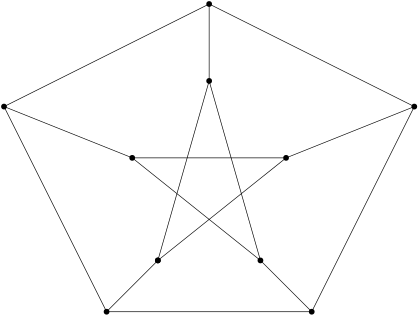
\includegraphics[width=0.5\linewidth]{img/opis-petersen.png}
    \caption{Petersenov graf}
\end{figure}
\end{zgled}

\newpage

\subsection*{Literatura}

\begin{itemize}
\item {\literatura G. Fijavž, \href{http://matematika.fri.uni-lj.si/ds/ds.pdf}{\emph{Diskretne strukture}}, elektronska knjiga, 2015.} 
\item {\literatura M. Juvan in P. Potočnik, \emph{Teorija grafov in kombinatorika}, DMFA-založništvo, Ljubljana 2000.}
\item {\literatura N. Prijatelj, \emph{Osnove matematične logike I}, DMFA-založništvo, Ljubljana, 1992.}
\end{itemize}

\chapter{Izjavni račun}

V tem poglavju si bomo pogledali, kako \emph{formaliziramo} preproste izjave in kako \emph{dokazujemo} njihovo veljavnost oziroma neveljavnost.

\section{Izjave in izjavni vezniki}

{\definicija Izjava} je poved, ki je bodisi resnična bodisi lažna.

\begin{zgled} \leavevmode
\begin{itemize}
    \item Ena in ena je tri. \emph{Lažna izjava.}
    \item Ena in ena je dve. \emph{Resnična izjava.}
    \item Koliko je ena in ena? \emph{Ni izjava.}
    \item Pojdimo na kavo! \emph{Ni izjava.}
\end{itemize}
\end{zgled}

Izjave lahko razdelimo na dve skupini \emph{po vsebini}, in sicer:
\begin{itemize}
    \item {\definicija resnične izjave}, ki imajo resničnostno vrednost $1$ ali $\top$ ali \texttt{true},
    \item {\definicija lažne izjave}, ki imajo resničnostno vrednost $0$ ali $\bot$ ali \texttt{false}.
\end{itemize}
Po \emph{zgradbi} oziroma \emph{obliki} pa izjave razdelimo na:
\begin{itemize}
    \item {\definicija osnovne}, ki ne vsebujejo izjavnih veznikov,
    \item {\definicija sestavljene}, ki vsebujejo izjavne veznike.
\end{itemize}

\begin{zgled} \leavevmode
\begin{itemize}
    \item Vreme je lepo. \emph{Osnovna izjava.}
    \item Špela gre v hribe. \emph{Osnovna izjava.}
    \item Vreme je lepo \emph{in} Špela gre v hribe. \emph{Sestavljena izjava.}
    \item \emph{Če} je vreme lepo, \emph{potem} gre Špela v hribe. \emph{Sestavljena izjava.}
    \item Špela \emph{ne} gre v hribe. \emph{Sestavljena izjava.}
\end{itemize}
\end{zgled}

Naj bo $n \in \NN_0$. {\definicija Izjavni veznik reda $n$} (ali {\definicija $n$-mestni izjavni veznik}) je funkcija, ki vsaki urejeni $n$-terici ničel in enic priredi vrednost $0$ ali $1$.

\begin{zgled} \leavevmode
\begin{itemize}
    \item Primer izjavnega veznika reda $1$ je {\definicija negacija}, ki $1$-terici $0$ priredi vrednost $1$, $1$-terici $1$ pa priredi vrednost $0$. Simbol za ta veznik je $\lnot$. Če je $p$ izjava, njeno negacijo označimo kot $\lnot p$ in preberemo kot \emph{ne $p$} ali kot \emph{ni res, da velja $p$}.
\end{itemize}
\end{zgled}

\section{Izjavni izrazi}
\section{Tavtologije in enakovredni izrazi}
\section{DNO in KNO}
\section{Sklepanje v izjavnem računu}
\section{Polni nabori izjavnih veznikov}


\chapter{Predikatni račun}
\chapter{Relacije}
\chapter{Urejenosti}
\chapter{Grafi}

$1$

\end{document}
